%
% latex-sample.tex
%
% This LaTeX source file provides a template for a typical research paper.
%

%
% Use the standard article template.
%
\documentclass{article}

% The geometry package allows for easy page formatting.
\usepackage{geometry}
\geometry{letterpaper}

% Load up special logo commands.
\usepackage{doc}

% Package for formatting URLs.
\usepackage{url}

% Packages and definitions for graphics files.
\usepackage{graphicx}
\usepackage{epstopdf}
\DeclareGraphicsRule{.tif}{png}{.png}{`convert #1 `dirname #1`/`basename #1 .tif`.png}

%
% Set the title, author, and date.
%
\title{An Ideal Headmaster Interface}
\author{Joseph Crawley}
\date{November 26, 2012}

%
% The document proper.
%
\begin{document}

% Add the title section.
\maketitle

% Add an abstract.
\abstract{}
As a website, Headmaster, a student database with information associated to each student, is very sleek and easy to use in its current form. However, a command line prompt which takes in simple English commands would be an ideal interface because it is easy to understand and users can access information quickly.

% Add various lists on new pages.
\pagebreak
\tableofcontents


%\listoffigures


%\listoftables

% Start the paper on a new page.
\pagebreak

%
% Body text.
%
\section{Explanation of Design}
\label{introduction}

When Headmaster is opened, the only thing to appear on the page is text that would say \begin{quote} What would you like to see? \end{quote}

The user would then enter a command in plain English of what they would want to see. The interface would then remove 
\centering
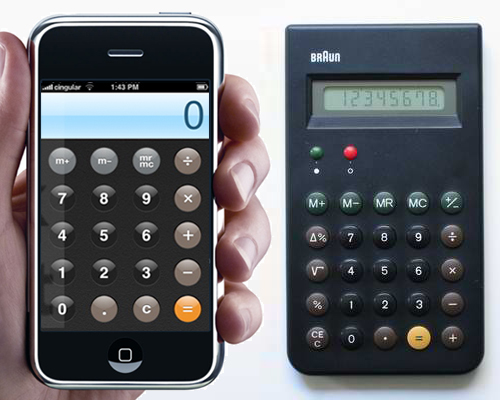
\includegraphics[width=2.5in]{calculator.jpeg} 

\caption{iPhone calculator compared to a physical calculator}
\label{calc}
\end{figure}

\section{Positives of Skeuomorphism}

Probably the biggest benefit of Skeuomorphs is that the design presents a low learning curve. This style of design is very intuitive for users, making the learnability of these interfaces fairly easy ~\cite{Former-UI}. For example in Figure~\ref{book}, the bookshelf application on the iPad is a very easy interface to understand. Reading books and magazines on the iPad is as simple as flipping a digital page like you would in an actual book. This design choice is something that is very intuitive and easy to pick up on. Also in general, skeuomorphs tend to be more aesthetically pleasing to the user. A sense of comfortability sweeps over the user. According to UCLA professor Nicholas Gessler, “They provide us with familiar cues to an unfamiliar domain.”~\cite{Gessler} When designers first tried to relate on-screen applications to users, files were stored in a virtual folder, and a virtual Rolodex stored the contacts. ~\cite{FastCompany3}
\begin{figure}
\centering
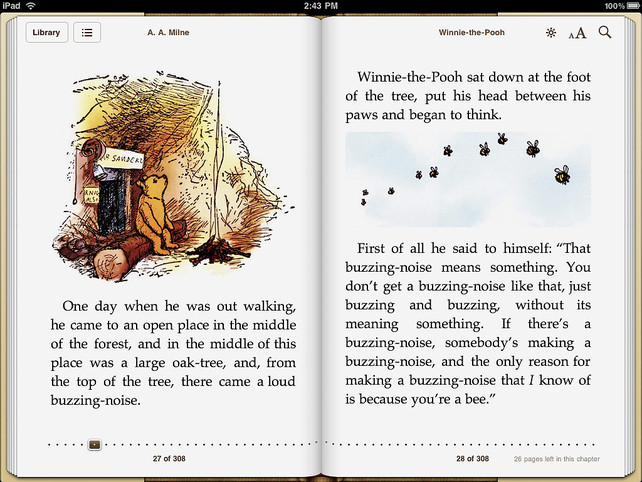
\includegraphics[width=2.5in]{ipadBook.jpeg} 

\caption{Winnie the Pooh on the iPad}
\label{book}
\end{figure}
\section{Arguments against Skeuomorphism}

In Apple’s Human Interface Guidelines, it says:

\begin{quote}Think of the objects and scenes you design as opportunities to communicate with users and to express the essence of your app. Don't feel that you must strive for scrupulous accuracy. Often, an amplified or enhanced portrayal of something can seem more real, and convey more meaning, than a faithful likeness.\end{quote}

In summary, this quote means that the best way to communicate with a user is to design the interface so that the function of the application is displayed ~\cite{Gizmodo}. In the following sections, I will highlight different skeuomorphic designs and talk about the flaws in the design.

\begin{table}
\centering
\begin{tabular}{|c|c|}\hline
Windows Metro & Classic Desktop \\\hline\hline
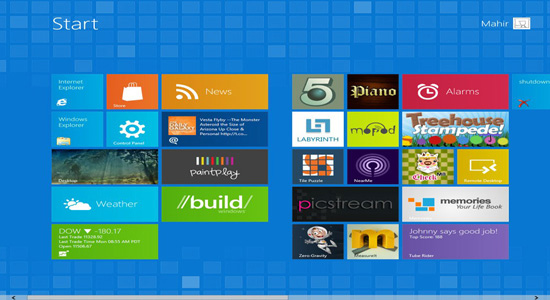
\includegraphics[width = 2.5in]{metro.jpeg} & 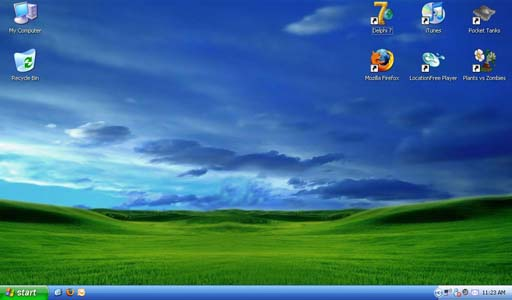
\includegraphics[width = 2.5in]{pc-desktop.jpeg} \\\hline
\end{tabular}

\caption{Two example desktops}
\label{desktops}
\end{table}

\subsection{The classic Desktop and Operating System Startup Screens}
	For years, computers desktops have mimicked the literal function of a desk. On a traditional computer, one would go to the desktop or home screen, and the icons would be laid out like papers spread out across a desk. Although this design is useful, desktops can often become cluttered and hard to manage almost like a messy desk. In the new Windows 8 operating system, Microsoft makes the home screen the “Metro” rather than the classic desktop. Although the Metro interface has its flaws and is far from perfect, it is essentially a more dynamic interface than the desktop. Home screens in operating systems are meant for users to be able to access their files and applications quickly. On the desktop, applications and files are organized by either when they were added to the desktop or to wherever the user designates them. On the Windows 8 Metro, the contrasting boxes and clear signage allows users to clearly organize and find the applications and files they need and use the most ~\cite{Hobbs}. The Metro interface strayed away from the traditional desk skeuomorph and made a design that featured accessibility. 


\subsection{Skeuomorphism and Usability Metrics}
	When studying user interfaces and interaction design, one will find that there are generally five metrics that experts agree on to effectively evaluate interfaces: 
\begin{itemize}
\item Learnability 
\item Memorability 
\item Efficiency 
\item Errors 
\item Satisfaction 
\end{itemize}

	Since skeuomorphic designs are familiar and intuitive, usually skeuomorphic designs should score high in the learnability and memorability. However when it comes to efficiency and errors, skeuomorphic designs may not always score highly. That is because when transferred across mediums, a skeuomorphic design is not always the best design. 
	\begin{emph}Many times, an interface that is effective when the object is physically accessed with fingers is not as efficient when that interface is portrayed on a screen and is accessed by a mouse and a keyboard. 
	\end{emph}
	
	Interfaces are most effective when designers allow the screen to act like a screen, rather than like paper. For example in Figure~\ref{Flipboard}, the Flipboard application on the iPad, the pages flip around the center of the page rather than on the left like a traditional book. This allows for easier, more efficient use for the users and is much more aesthetically pleasing.~\cite{wired}
\begin{figure}
\centering
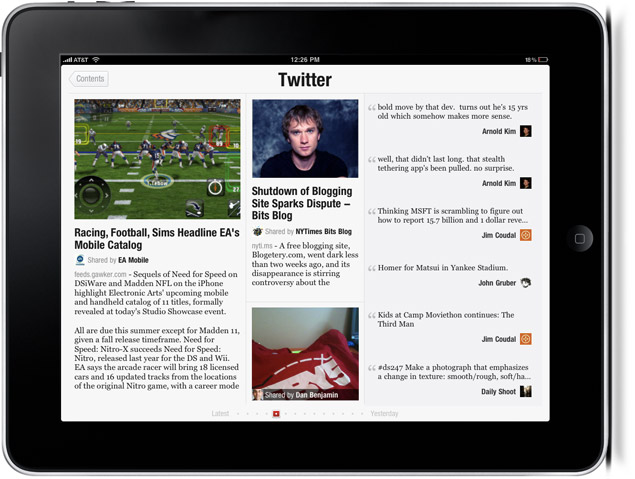
\includegraphics[width=2.5in]{flipboard.jpeg} 

\caption{Flipboard application for the iPad}
\label{Flipboard}
\end{figure}

\begin{figure}
\centering
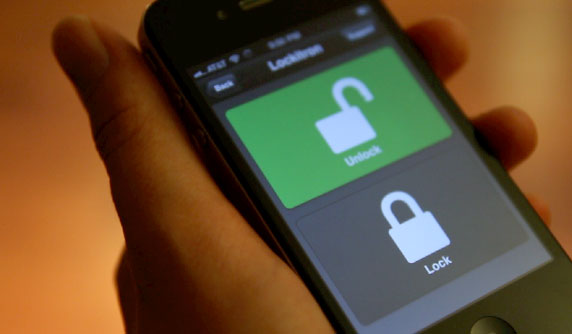
\includegraphics[width=2.5in]{lockitron.jpeg} 

\caption{Lockitron}
\label{Lockitron Smartphone App}
\end{figure}
\subsection{Skeuomorphism and Evolutionary Design}

At times, the skeuomorphic design is not always the best design for an interface. For example, there is a smartphone application called Lockitron which allows users to lock their front doors will a simple push of a button. Imagine if instead of just pushing a button to unlock the door, the user would have to turn a virtual key. The act of turning a virtual key is cumbersome and less efficient then simply pressing an unlock button. New design techniques have evolved the science of design and enhanced the user experience in technology. The design of things like the modern computer mouse and the iPod scroll wheel has made technology more efficient and user friendly ~\cite{ipod}. The mouse and the scroll wheel were not skeuomorphs, and accessibility and usability continues to grow with the enhancement of touch and voice technology. 



\section{Conclusion}

	After doing research, I believe that skeuomorphs do have a place in interaction design. Skeuomorphs bring a sense of comfort, but should be used in moderation. When transferring an interface from the physical medium to a technology, the appearance of an object should resemble its behavior. For example, in the new operating system for Macs, the address book appears like a leather-bound journal, but doesn’t have the pages like a journal does. The most intuitive, instinctual design, may not always be the best design.
\pagebreak
% Generate the bibliography.
\bibliography{intro}
\bibliographystyle{plain}

\end{document}
